\documentclass[../main.tex]{subfiles}






\begin{document}
\chapter{}
\label{cha:cha_16}

\section{}
A table of integrals can be consulted to determine
	\bigbreak
$\displaystyle\int \tanh d x=\dfrac{1}{a} \ln \cosh a x$
	\bigbreak
Therefore,
	\bigbreak
$\displaystyle\int_{0}^{t} \sqrt{\dfrac{g m}{c_{d}}} \tanh \left(\sqrt{\dfrac{g c_{d}}{m} t}\right) d t=\sqrt{\dfrac{g m}{c_{d}}} \sqrt{\dfrac{m}{g c_{d}}}\left[\operatorname { l n } \operatorname { c o s h } \left(\sqrt{\dfrac{g c_{d}}{m}} t\right)\right]^{t}_{0}$
	\bigbreak
$\sqrt{\dfrac{g m^{2}}{g c_{d}^{2}}}\left[\ln \cosh \left(\sqrt{\dfrac{g c_{d}}{m}} t\right)-\ln \cosh (0)\right]$
	\bigbreak
Since cosh(0) = 1 and ln(1) = 0, this reduces to
	\bigbreak
$\dfrac{m}{c_{d}} \ln \cosh \left(\sqrt{\dfrac{g c_{d}}{m}} t\right)$
	\bigbreak



\section{}
\begin{enumerate}[label=\bfseries(\alph*)]
\item the analytical solution can be evaluated as
	\bigbreak
$\displaystyle\int_{0}^{4}\left(1-e^{-2 x}\right) d x=\left[x+0.5 e^{-2 x}\right]_{0}^{4}=4+0.5 e^{-2(4)}-0-0.5 e^{-2(0)}=3.500167731$
	\bigbreak
\item single application of the trapezoidal rule 
	\bigbreak
$(4-0) \dfrac{0+0.999665}{2}=1.99329 \quad\left(\epsilon_{t}=42.88 \%\right)$
	\bigbreak
\item composite trapezoidal rule
	\bigbreak
$n=2:$
	\bigbreak
$(4-0) \dfrac{0+2(0.981684)+0.999665}{4}=2.96303 \quad\left(\epsilon_{t}=15.35 \%\right)$
	\bigbreak
$n=4:$
	\bigbreak
$(4-0) \dfrac{0+2(0.86466+0.981684+0.99752)+0.999665}{8}=3.3437 \quad\left(\epsilon_{t}=4.47 \%\right)$
	\bigbreak
\item single application of Simpson’s 1/3 rule 
	\bigbreak
$(4-0) \dfrac{0+4(0.981684)+0.999665}{6}=3.28427 \quad\left(\epsilon_{t}=6.17 \%\right)$
	\bigbreak
\item composite Simpson’s 1/3 rule (n = 4) 
	\bigbreak
$(4-0) \dfrac{0+4(0.86466+0.99752)+2(0.981684)+0.999665}{12}=3.47059 \quad\left(\epsilon_{t}=0.84 \%\right)$
	\bigbreak
\item Simpson’s 3/8 rule
	\bigbreak
$(4-0) \dfrac{0+3(0.930517+0.995172)+0.999665}{8}=3.388365 \quad\left(\epsilon_{t}=3.19 \%\right)$
	\bigbreak
\end{enumerate}



\section{}
\begin{enumerate}[label=\bfseries(\alph*)]
\item the analytical solution can be evaluated as
	\bigbreak
$\displaystyle\int_{0}^{\pi / 2}(6+3 \cos x) d x=[6 x+3 \sin x]_{0}^{\pi / 2}=6(\pi / 2)+3 \sin (\pi / 2)-6(0)-3 \sin (0)=12.424778$
	\bigbreak

\item single application of the trapezoidal rule
	\bigbreak
$\left(\dfrac{\pi}{2}-0\right) \dfrac{9+6}{2}=11.78097 \quad\left(\epsilon_{t}=5.18 \%\right)$
	\bigbreak

\item composite trapezoidal rule
	\bigbreak
$n=2:$
	\bigbreak
$\left(\dfrac{\pi}{2}-0\right) \dfrac{9+2(8.12132)+6}{4}=12.26896 \quad\left(\epsilon_{t}=1.25 \%\right)$
	\bigbreak
$n=4:$
	\bigbreak
$\left(\dfrac{\pi}{2}-0\right) \dfrac{9+2(8.77164+8.12132+7.14805)+6}{8}=12.386125 \quad\left(\epsilon_{t}=0.3111 \%\right)$

\item single application of Simpson’s 1/3 rule
	\bigbreak
$\left(\dfrac{\pi}{2}-0\right) \dfrac{9+4(8.12132)+6}{6}=12.4316 \quad\left(\epsilon_{t}=0.0550 \%\right)$
	\bigbreak

\item composite Simpson’s 1/3 rule (n = 4)
	\bigbreak
$\left(\dfrac{\pi}{2}-0\right) \dfrac{9+4(8.7716+7.14805)+2(8.12132)+6}{12}=12.42518 \quad\left(\epsilon_{t}=0.0032 \%\right)$
	\bigbreak

\item Simpson’s 3/8 rule
	\bigbreak
$\left(\dfrac{\pi}{2}-0\right) \dfrac{9+3(8.59808+7.5)+6}{8}=12.42779 \quad\left(\epsilon_{t}=0.0243 \%\right)$
	\bigbreak 
\end{enumerate}



\section{}
\begin{enumerate}[label=\bfseries(\alph*)]
\item the analytical solution can be evaluated as
	\bigbreak
$\displaystyle\int_{-2}^{4} \left(1-x-4 x^{3}+2 x^{5}\right) d x=\left[x-\dfrac{x^{2}}{2}-x^{4}+\dfrac{x^{6}}{3}\right]_{-2}^{4}$
	\bigbreak
$=4-\dfrac{4^{2}}{2}-4^{4}+\dfrac{4^{6}}{3}-(-2)+\dfrac{(-2)^{2}}{2}+(-2)^{4}-\dfrac{(-2)^{6}}{3}=1104$
	\bigbreak
\item single application of the trapezoidal rule
	\bigbreak
$(4-(-2)) \dfrac{-29+1789}{2}=5280 \quad\left(\epsilon_{t}=378.3 \%\right)$
	\bigbreak

\item composite trapezoidal rule
	\bigbreak
$n=2:$
	\bigbreak
$(4-(-2)) \dfrac{-29+2(-2)+1789}{4}=2634 \quad\left(\epsilon_{t}=138.6 \%\right)$
	\bigbreak
$n=4:$
	\bigbreak
$(4-(-2)) \dfrac{-29+2(1.9375+(-2)+131.3125)+1789}{8}=1516.875 \quad\left(\epsilon_{t}=37.4 \%\right)$
	\bigbreak

\item single application of Simpson’s 1/3 rule
	\bigbreak
$(4-(-2)) \dfrac{-29+4(-2)+1789}{6}=1752 \quad\left(\epsilon_{t}=58.7 \%\right)$
	\bigbreak

\item composite Simpson’s 1/3 rule (n = 4)
	\bigbreak
$(4-(-2)) \dfrac{-29+4(1.9375+131.3125)+2(-2)+1789}{12}=1144.5 \quad\left(\epsilon_{t}=3.6685 \%\right)$
	\bigbreak

\item Simpson’s 3/8 rule
	\bigbreak
$(4-(-2)) \dfrac{-29+3(1+31)+1789}{8}=1392 \quad\left(\epsilon_{t}=26.09 \%\right)$
	\bigbreak

\item Boole's rule.
	\bigbreak
$(4-(-2)) \dfrac{7(-29)+32(1.9375)+12(-2)+32(131.3125)+7(1789)}{90}=1104 \quad\left(\epsilon_{t}=0 \%\right)$
	\bigbreak 
\end{enumerate}



\section{}
\begin{enumerate}[label=\bfseries(\alph*)]
\item The analytical solution can be evaluated as
	\bigbreak
$\displaystyle\int_{0}^{1.2} e^{-x} d x=\left[-e^{-x}\right]_{0}^{1.2}=-e^{-1.2}-\left(-e^{0}\right)=0.69880579$
	\bigbreak

\item  Trapezoidal rule
	\bigbreak
$(0.1-0) \dfrac{1+0.90484}{2}+(0.3-0.1) \dfrac{0.90484+0.74082}{2}+(0.5-0.3) \dfrac{0.74082+0.60653}{2}$
	\bigbreak
$+(0.7-0.5) \dfrac{0.60653+0.49659}{2}+(0.95-0.7) \dfrac{0.49659+0.38674}{2}+(1.2-0.957) \dfrac{0.38674+0.30119}{2}$
	\bigbreak
$=0.09524+0.164566+0.134735+0.110312+0.110416+0.085992=0.70126\left(\epsilon_{t}=0.35 \%\right)$
	\bigbreak

\item Trapezoidal and Simpson’s Rules
	\bigbreak
$(0.1-0) \dfrac{1+0.90484}{2}+(0.7-0.1) \dfrac{0.90484+3(0.74082+0.60653)+0.49659}{8}$
	\bigbreak
$+(1.2-0.7) \dfrac{0.49659+4(0.38674)+0.30119}{6}=0.09524+0.40826+0.195395=0.698897\left(\epsilon_{t}=0.0131 \%\right)$ 
	\bigbreak
\end{enumerate}



\section{}
\begin{enumerate}[label=\bfseries(\alph*)]
\item The integral can be evaluated analytically as,
	\bigbreak

$\displaystyle\int_{-2}^{2}\left[\dfrac{x^{3}}{3}-3 y^{2} x+y^{3} \dfrac{x^{2}}{2}\right]_{0}^{4} d y$ \bigbreak
$\displaystyle\int_{-2}^{2} \dfrac{(4)^{3}}{3}-3 y^{2}(4)+y^{3} \dfrac{(4)^{2}}{2} d y$ \bigbreak
$\displaystyle\int_{-2}^{2} 21.33333-12 y^{2}+8 y^{3} d y$ \bigbreak
${\left[21.33333 y-4 y^{3}+2 y^{4}\right]_{-2}^{2}}$ \bigbreak
$21.33333(2)-4(2)^{3}+2(2)^{4}-21.33333(-2)+4(-2)^{3}-2(-2)^{4}=21.33333$ \bigbreak

\item The composite trapezoidal rule with n = 2 can be used the evaluate the inner integral at
the three equispaced values of y,
	\bigbreak
$y=-2: \quad(4-0) \dfrac{-12+2(-24)-28}{4}=-88$ \bigbreak
$y=0: \quad(4-0) \dfrac{0+2(4)+16}{4}=24$ \bigbreak
$y=2: \quad(4-0) \dfrac{-12+2(8)+36}{4}=40$ \bigbreak

These results can then be integrated in y to yield
	\bigbreak
$(2-(-2)) \dfrac{-88+2(24)+40}{4}=0$
	\bigbreak
which represents a percent relative error of
	\bigbreak
$\epsilon_{t}=\left|\dfrac{21.33333-0}{21.33333}\right| \times 100 \%=100 \%$ 
	\bigbreak
which is not very good.
	\bigbreak

\item Single applications of Simpson’s 1/3 rule can be used the evaluate the inner integral at
the three equispaced values of y,
	\bigbreak
$
\begin{array}{ll}
y=-2: & (4-0) \dfrac{-12+4(-24)-28}{6}=-90.66667 \\
y=0: & (4-0) \dfrac{0+4(4)+16}{6}=21.33333 \\
y=2: & (4-0) \dfrac{-12+4(8)+36}{6}=37.33333
\end{array}
$
	\bigbreak
These results can then be integrated in y to yield
	\bigbreak
$(2-(-2)) \dfrac{-90.66667+4(21.33333)+37.33333}{6}=21.33333$
	\bigbreak
which represents a percent relative error of
	\bigbreak
$\epsilon_{t}=\left|\dfrac{21.33333-21.33333}{21.33333}\right| \times 100 \%=0 \%$
	\bigbreak
which is perfect
	\bigbreak
\end{enumerate}



\section{}
\begin{enumerate}[label=\bfseries(\alph*)]
\item The integral can be evaluated analytically as,
	\bigbreak
$\displaystyle\int_{-4}^{4} \int_{0}^{6}\left[\dfrac{x^{4}}{4}-2 y z x\right]_{-1}^{3} d y d z=\int_{-4}^{4} \int_{0}^{6} 20-8 y z d y d z$
	\bigbreak
$\displaystyle\int_{-4}^{4} \int_{0}^{6} 20-8 y z d y d z=\int_{-4}^{4}\left[20 y-4 z y^{2}\right]_{0}^{6} d z=\int_{-4}^{4} 120-144 z d z$
	\bigbreak
$\displaystyle\int_{-4}^{4} 120-144 z d z=\left[120 z-72 z^{2}\right]_{-4}^{4}=120(4)-72(4)^{2}-120(-4)+72(-4)^{2}=960$
	\bigbreak
\item Single applications of Simpson's $1 / 3$ rule can be used the evaluate the inner integral at the three equispaced values of $y$ for each value of $z$,
	\bigbreak
z=-4:
	\bigbreak
$y=0: \quad(3-(-1)) \dfrac{-1+4(1)+27}{6}=20$
	\bigbreak
$y=3: \quad(3-(-1)) \dfrac{23+4(25)+51}{6}=116$
	\bigbreak
$y=6: \quad(3-(-1)) \dfrac{47+4(49)+75}{6}=212$
	\bigbreak
These results can then be integrated in $y$ to yield
	\bigbreak
$(6-0) \dfrac{20+4(116)+212}{6}=696$
	\bigbreak
z=0:
	\bigbreak
$y=0: \quad(3-(-1)) \dfrac{-1+4(1)+27}{6}=20$
	\bigbreak
$y=3: \quad(3-(-1)) \dfrac{-1+4(1)+27}{6}=20$
	\bigbreak
$y=6: \quad(3-(-1)) \dfrac{-1+4(1)+27}{6}=20$
	\bigbreak
These results can then be integrated in $y$ to yield
	\bigbreak
$(6-0) \dfrac{20+4(20)+20}{6}=120$
	\bigbreak
z=4:
	\bigbreak
$y=0: \quad(3-(-1)) \dfrac{-1+4(1)+27}{6}=20$
	\bigbreak
$y=3: \quad(3-(-1)) \dfrac{-25+4(-23)+3}{6}=-76$
	\bigbreak
$y=6: \quad(3-(-1)) \dfrac{-49+4(-47)-21}{6}=-172$
	\bigbreak
These results can then be integrated in $y$ to yield
	\bigbreak
$(6-0) \dfrac{20+4(-76)-172}{6}=-456$
	\bigbreak
The results of the integrations in $y$ can then be integrated in $z$ to yield
	\bigbreak
$(6-0) \dfrac{696+4(120)-456}{6}=960$
	\bigbreak
which represents a percent relative error of
	\bigbreak
$\varepsilon_{t}=\left|\dfrac{960-960}{960}\right| \times 100 \%=0 \%$
\end{enumerate}



\section{}
\begin{enumerate}[label=\bfseries(\alph*)]
\item The trapezoidal rule can be implemented as,
	\bigbreak
$d=(2-1) \dfrac{5+6}{2}+(3.25-2) \dfrac{6+5.5}{2}+(4.5-3.25) \dfrac{5.5+7}{2}+(6-4.5) \dfrac{7+8.5}{2}$
	\bigbreak
$+(7-6) \dfrac{8.5+6}{2}+(8-7) \dfrac{6+6}{2}+(8.5-8) \dfrac{6+7}{2}+(9.3-8.5) \dfrac{7+7}{2}+(10-9.3) \dfrac{7+5}{2}=58.425$
	\bigbreak
\item  The polynomial can be fit as,
	\bigbreak
\begin{lstlisting}[numbers=none]
>> format long
>> t = [1 2 3.25 4.5 6 7 8 8.5 9.3 10];
>> v = [5 6 5.5 7 8.5 6 6 7 7 5];
>> p = polyfit(t,v,3)


p =
	-0.00657842294444	0.01874733808337	0.56859435273356
4.46645555949356 
\end{lstlisting}
	\bigbreak
The cubic can be plotted along with the data,
	\bigbreak
\begin{lstlisting}[numbers=none]
>> tt = linspace(1,10);
>> vv = polyval(p,tt);
>> plot(tt,vv,t,v,'o') 
\end{lstlisting}
	\bigbreak
	\begin{figure}[H]
		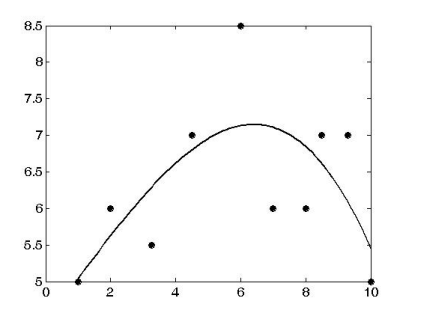
\includegraphics[width=0.5\linewidth]{fig_16_1}
		\label{fig:fig_16_1}
	\end{figure}
	\bigbreak
The cubic can then be integrated to estimate the distance traveled,
	\bigbreak
$
\begin{aligned}
&d =\int_{1}^{10}-0.006578 t^{3}+0.018747 t^{2}+0.568594 t+4.46646 d t \\
&=\left[-0.001645 t^{4}+0.006249 t^{3}+0.284297 t^{2}+4.46646 t\right]_{1}^{10}=58.14199
\end{aligned}
$
\end{enumerate}
	\bigbreak



\section{}
\begin{tabular}{rrrr}
\hline
$z$ & $w(z)$ & $\rho g w(z)(60-z)$ & $\rho g z w(z)(60-z)$ \\
\hline
60 & 200 & 0 & 0 \\
50 & 190 & $1.8639 E+07$ & $9.3195 \mathrm{E}+08$ \\
40 & 175 & $3.4335 \mathrm{E}+07$ & $1.3734 \mathrm{E}+09$ \\
30 & 160 & $4.7088 \mathrm{E}+07$ & $1.4126 \mathrm{E}+09$ \\
20 & 135 & $5.2974 \mathrm{E}+07$ & $1.0595 \mathrm{E}+09$ \\
10 & 130 & $6.3765 \mathrm{E}+07$ & $6.3765 \mathrm{E}+08$ \\
0 & 122 & $7.1809 \mathrm{E}+07$ & 0 \\
\hline
\end{tabular}
	\bigbreak
$f_{t}=60 \dfrac{7.1809+4(6.3765+4.7088+1.8639)+2(5.2974+3.4335)+0}{3(6)} \times 10^{7}=2.5480 \times 10^{9}$
	\bigbreak
$\displaystyle\int_{0}^{D} \rho g z w(z)(D-z) d z=60 \dfrac{0+4(0.63765+1.4126+0.93195)+2(1.0595+1.3734)+0}{3(6)} \times 10^{9}=5.5982 \times 10$
	\bigbreak
$d=\dfrac{5.5982 \times 10^{10}}{2.5480 \times 10^{9}}=21.971$
	\bigbreak


\section{}
\begin{enumerate}[label=\bfseries(\alph*)]
\item Trapezoidal rule:
	\bigbreak
$f=30 \dfrac{0+2(54.937+51.129+36.069+27.982+19.455)+13.311}{2(6)}=996.1363$
	\bigbreak
$f=\dfrac{30 \dfrac{0+2(274.684+511.292+586.033+559.631+486.385)+399.332}{2(6)}}{996.1363}=\dfrac{13088.45}{996.1363}=13.139 \mathrm{~m}$
	\bigbreak
\item Simpson's 1/3 rule:
	\bigbreak
$
\begin{gathered}
f=30 \dfrac{0+4(54.937+36.069+19.455)+2(51.129+27.982)+13.311}{3(6)}=1042.294 \\
30 \dfrac{0+4(274.684+586.033+486.385)+2(511.292+559.631)+399.332}{3(6)}=\dfrac{13215.97}{1042.294}=12.6797 \mathrm{~m}
\end{gathered}
$
	\bigbreak
\end{enumerate}
\end{document}